\section{Resultat}

Vid redovisningstillfället slutfördes två körningar på 15 varv vardera där de
fem första var kalibreringsvarv (enligt krav 20 och 22). Vid den första
körningen var referenstiden inställd på 13 sekunder och vid den andra var
referenstiden inställd på 14 sekunder. De två körningarna finns uppritade i
Figur~\ref{fig:laptimes-calibration} med kalibreringsvarven och i Figur~
\ref{fig:laptimes-no-calibration} utan kalibreringsvarven med vald referenstid
och den maximalt tillåtna avvikelsen på 0,5 sekunder (enligt krav 21) inritat.
Figur~\ref{fig:segtimes} visar den genomsnittliga segmentstiden vid vardera
körning och Tabell~\ref{table:resultat} visar resultaten beskrivna nedan.

Vid den första körningen höll bilen en genomsnittlig varvtid på 13,22~sekunder
med en standardavvikelse på 0,24~sekunder. $\pm$0,5~sekunder överträddes vid två
av varven med varvtider på 13,54 och 13,52~sekunder. Vid den andra körningen höll bilen en genomsnittlig varvtid på 14,47~sekunder
med en standardavvikelse på 0,26~sekunder. $\pm$0,5~sekunder överträddes vid
fyra av varven med en maximal överträdelse på 0,31~sekunder långsammare än
maximal tillåten varvtid (14,5~sekunder).

Ingen av dessa körningar uppfyllde kraven på prestanda, alltså krav 20, 21 och
23. Givarna lästes av mer än 10 gånger per sekund under båda körningarna. Se
\ref{sec:system:korning:cykel} för information om hur detta mäts.

\begin{figure}
	\centering
	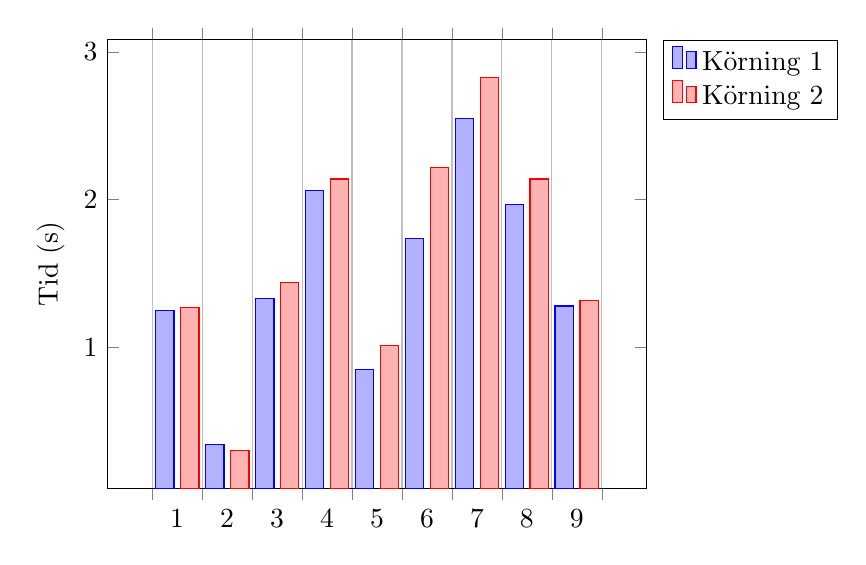
\begin{tikzpicture}
		\begin{axis} [
				ylabel=Tid (s),
				legend pos = outer north east,
				ybar interval=0.75
		]
			\addplot+ [] coordinates {(1, 1.25) (2, 0.34) (3, 1.33) (4, 2.06) (5, 0.85)
			(6, 1.74) (7, 2.55) (8, 1.97) (9, 1.28) (10, 1)};
			\addlegendentry{Körning 1}
			\addplot+ [] coordinates {(1, 1.27) (2, 0.30) (3, 1.44) (4, 2.14) (5, 1.01)
			(6, 2.22) (7, 2.83) (8, 2.14) (9, 1.32) (10, 1)};
			\addlegendentry{Körning 2}
		\end{axis}
	\end{tikzpicture}
	\caption{Genomsnittlig segmentstid för de två körningarna från redovisningen.}
	\label{fig:segtimes}
\end{figure}

\begin{table}
	\centering
	\caption{Resultaten från de två körningarna.}
	\begin{tabular}{|c|c|c|c|}
		\hline
		Körning & Referenstid & Snitt & Standardavvikelse \\\hline
		1 & 13 & 13,22 & 0,24 \\\hline
		2 & 14 & 14,47 & 0,26 \\\hline
	\end{tabular}
	\label{table:resultat}
\end{table}

\begin{figure}
	\centering

	\begin{tikzpicture}
		\begin{axis} [xmin=0, xmax=15.5,ymin=10,ymax=20, xlabel=Varv, ylabel={Tid (s)}, 
						legend pos=outer north east]
			\addplot+ [blue, mark options={blue}, mark=square*] table [col sep=comma, x index=0, y index = 1] {stats/lap.csv};
			\addlegendentry{Körning 1}
			\addplot+ [red, mark options={red}, mark=*] table [col sep=comma, x index=0, y index = 2] {stats/lap.csv};
			\addlegendentry{Körning 2}
		\end{axis}
	\end{tikzpicture}
  \caption{Varvtider för de två körningarna från redovisningen, inklusive
	kalibreringsvarven.}
	\label{fig:laptimes-calibration}

	\vspace*{\floatsep}% https://tex.stackexchange.com/q/26521/5764

	\begin{tikzpicture}
		\begin{axis} [xmin=5.5, xmax=15.5,ymin=12,ymax=16, xlabel=Varv, ylabel={Tid (s)}, 
						legend pos=outer north east]
			\addplot+ [blue, mark options={blue}, mark=square*] table [col sep=comma, x index=0, y index = 1] {stats/lap.csv};
			\addlegendentry{Körning 1}
			\addplot[blue, domain=0:20] {13};
			\addlegendentry{Referenstid körning 1}
			\addplot+ [red, mark options={red}, mark=*] table [col sep=comma, x index=0, y index = 2] {stats/lap.csv};
			\addlegendentry{Körning 2}
			\addplot [red, domain=0:20] {14};
			\addlegendentry{Referenstid körning 2}
			\draw[dotted] (axis cs:0,12.5) -- (axis cs:16,12.5);
			\draw[dotted] (axis cs:0,13.5) -- (axis cs:16,13.5);
			\draw[dotted] (axis cs:0,14.5) -- (axis cs:16,14.5);
		\end{axis}
	\end{tikzpicture}
	\caption{Varvtider för de två körningarna från redovisningen, exklusive
	kalibreringsvarven.}
	\label{fig:laptimes-no-calibration}
\end{figure}
